\documentclass[a4paper,twoside,zihao=5,UTF8]{ctexart}

\ctexset{
	section = {
		format+ = \zihao{-4} \heiti \raggedright,
		name = {,、},
		number = \chinese{section},
		beforeskip = 1.0ex plus 0.2ex minus .2ex,
		afterskip = 1.0ex plus 0.2ex minus .2ex,
		aftername = \hspace{0pt}
	},
	subsection = {
		format+ = \zihao{5} \heiti \raggedright,
		name = {\thesubsection、},
		name = {,、},
		number = \arabic{subsection},
		beforeskip = 1.0ex plus 0.2ex minus .2ex,
		afterskip = 1.0ex plus 0.2ex minus .2ex,
		aftername = \hspace{0pt}
	}
}

\usepackage{blindtext}  
\usepackage{geometry}

% Page margin layout
\geometry{left=2.3cm,right=2cm,top=2.5cm,bottom=2.0cm}


\usepackage{listings}
\usepackage{xcolor}
\usepackage{geometry}
\usepackage{amsmath}
\usepackage{float}
\usepackage{hyperref}

\usepackage{graphics}
\usepackage{graphicx}
\usepackage{subfigure}
\usepackage{epsfig}
\usepackage{float}

\usepackage{algorithm}
\usepackage[noend]{algpseudocode}

\usepackage{booktabs}
\usepackage{threeparttable}
\usepackage{longtable}
\usepackage{listings}
\usepackage{tikz}
\usepackage{multicol}

% cite package, to clean up citations in the main text. Do not remove.
\usepackage{cite}

\usepackage{color,xcolor}

%% The amssymb package provides various useful mathematical symbols
\usepackage{amssymb}
%% The amsthm package provides extended theorem environments
\usepackage{amsthm}
\usepackage{amsfonts}
\usepackage{enumerate}
\usepackage{enumitem}
\usepackage{listings}

\usepackage{indentfirst}
\setlength{\parindent}{2em} % Make two letter space in the first paragraph
\usepackage{setspace}
\linespread{1.5} % Line spacing setting
\usepackage{siunitx}
\setlength{\parskip}{0.5em} % Paragraph spacing setting

% \usepackage[contents =22920202204622, scale = 10, color = black, angle = 50, opacity = .10]{background}

\renewcommand{\figurename}{图}
\renewcommand{\lstlistingname}{代码} 
\renewcommand{\tablename}{表格}
\renewcommand{\contentsname}{目录}
\floatname{algorithm}{算法}

\graphicspath{ {images/} }

%%%%%%%%%%%%%
\newcommand{\StudentNumber}{22920202204622}  % Fill your student number here
\newcommand{\StudentName}{熊恪峥}  % Replace your name here
\newcommand{\PaperTitle}{电子工艺实训}  % Change your paper title here
\newcommand{\PaperType}{实验报告} % Replace the type of your report here
\newcommand{\Date}{2022年6月27日至2022年7月8日}
\newcommand{\Grade}{2020级}
\newcommand{\Department}{计算机科学系}
%%%%%%%%%%%%%

%% Page header and footer setting
\usepackage{fancyhdr}
\usepackage{lastpage}
\pagestyle{fancy}
\fancyhf{}
% This requires the document to be twoside
\fancyhead[LO]{\texttt{\StudentName }}
\fancyhead[LE]{\texttt{\StudentNumber}}
\fancyhead[C]{\texttt{\PaperTitle }}
\fancyhead[R]{\texttt{第{\thepage}页,共\pageref*{LastPage}页}}


\title{\PaperTitle}
\author{\StudentName}
\date{\Date}

\lstset{
	basicstyle          =   \sffamily,          % 基本代码风格
	keywordstyle        =   \bfseries,          % 关键字风格
	commentstyle        =   \rmfamily\itshape,  % 注释的风格,斜体
	stringstyle         =   \ttfamily,  % 字符串风格
	flexiblecolumns,                % 别问为什么,加上这个
	numbers             =   left,   % 行号的位置在左边
	showspaces          =   false,  % 是否显示空格,显示了有点乱,所以不现实了
	numberstyle         =   \zihao{-5}\ttfamily,    % 行号的样式,小五号,tt等宽字体
	showstringspaces    =   false,
	captionpos          =   t,      % 这段代码的名字所呈现的位置,t指的是top上面
	frame               =   lrtb,   % 显示边框
}

\lstdefinestyle{PythonStyle}{
	language        =   Python, % 语言选Python
	basicstyle      =   \zihao{-5}\ttfamily,
	numberstyle     =   \zihao{-5}\ttfamily,
	keywordstyle    =   \color{blue},
	keywordstyle    =   [2] \color{teal},
	stringstyle     =   \color{magenta},
	commentstyle    =   \color{red}\ttfamily,
	breaklines      =   true,   % 自动换行,建议不要写太长的行
	columns         =   fixed,  % 如果不加这一句,字间距就不固定,很丑,必须加
	basewidth       =   0.5em,
}

\lstdefinestyle{CppStyle}{
	language        =   c++,
	basicstyle      =   \zihao{-5}\ttfamily,
	numberstyle     =   \zihao{-5}\ttfamily,
	keywordstyle    =   \color{blue},
	keywordstyle    =   [2] \color{teal},
	stringstyle     =   \color{magenta},
	commentstyle    =   \color{red}\ttfamily,
	breaklines      =   true,   % 自动换行,建议不要写太长的行
	columns         =   fixed,  % 如果不加这一句,字间距就不固定,很丑,必须加
	basewidth       =   0.5em,
}

\algnewcommand\algorithmicinput{\textbf{Input:}}
\algnewcommand\algorithmicoutput{\textbf{Output:}}
\algnewcommand\Input{\item[\algorithmicinput]}%
\algnewcommand\Output{\item[\algorithmicoutput]}%

\usetikzlibrary{positioning, shapes.geometric}

\begin{document}
	
%%%%%%%%%%%%%%%%%%%%%%%%%%%%%%%%%%%%%%%%%%%%
\makeatletter % change default title style
\renewcommand*\maketitle{%
	\begin{center} 
		\bfseries  % title 
		{\LARGE \@title \par}  % LARGE typesetting
		\vskip 1em  %  margin 1em
		{\global\let\author\@empty}  % no author information
		{\global\let\date\@empty}  % no date
		\thispagestyle{empty}   %  empty page style
	\end{center}%
	\setcounter{footnote}{0}%
}
\makeatother
%%%%%%%%%%%%%%%%%%%%%%%%%%%%%%%%%%%%%%%%%%%%
	
	
\thispagestyle{empty}

\vspace*{1cm}

\begin{figure}[h]
	\centering
	
\includegraphics[width=8.0cm]{logo.png}
\end{figure}

\vspace*{1cm}

\begin{center}
	\Huge{\textbf{\PaperType}}
	
	\Large{\PaperTitle}
\end{center}

\vspace*{1cm}

\begin{table}[h]
	\centering	
	\begin{Large}
		\renewcommand{\arraystretch}{1.5}
		\begin{tabular}{p{3cm} p{5cm}<{\centering}}
			姓\qquad 名 & \StudentName  \\
			\hline
			学\qquad号 & \StudentNumber \\
			\hline
			日\qquad期 & \Date  \\
			\hline
			年\qquad级 & \Grade  \\
			\hline
			系\qquad别 & \Department  \\
			\hline
		\end{tabular}
	\end{Large}
\end{table}

\newpage

\title{
	\Large{\textcolor{black}{\PaperTitle}}
}
	
	
\maketitle

\begin{center}
	姓名:\StudentName \qquad 学号:\StudentNumber \qquad 总分:
\end{center}
	
\tableofcontents
 
\newpage
\setcounter{page}{1}

\begin{spacing}{1.2}

\section{PCB制作部分}

\subsection{PCB设计过程及遇到的主要问题}

PCB制作过程和遇到的问题如表~\ref{tbl:pcb}。

\begin{table}[htbp]
	\renewcommand\arraystretch{1.5}
	\centering
	\caption{PCB制作过程和遇到的问题}
	\label{tbl:pcb}
	\begin{tabular}{p{4cm}|p{8cm}}
		\toprule
		\hline
		制作过程 & 问题 \\
		\hline
		原理图绘制 & \begin{minipage}[t]{8cm}
			\begin{enumerate}
				\item 在绘制原理图时连线有虚接的现象。
				\item 没有连接到正确的端口。
			\end{enumerate}
		\end{minipage} 
		
		\\
		\hline
		封装 & \begin{minipage}[t]{8cm}
			\begin{enumerate}
				\item 某些封装没有注意尺寸问题,使得原件安装困难。
				\item 有些封装没有明显标注正负极性,导致安装的时候翻查原理图。
			\end{enumerate}
		\end{minipage} 
		
		\\
		\hline
		布线 & \begin{minipage}[t]{8cm}
			\begin{enumerate}
				\item 没有注意线宽导致线过细,之后进行了修改
				\item 在保证无锐角、无重合的时候遇到了困难,之后重新调整了原件布置顺序
				\item 开关的引脚尺寸不合适
			\end{enumerate}
		\end{minipage} 

		\\
		\hline
		布局 & \begin{minipage}[t]{8cm}
			\begin{enumerate}
				\item 有些部分没有为安装预留足够的空隙
				\item 没有留够助焊区域使得焊接困难
			\end{enumerate}
		\end{minipage} 

		\\
		\hline
		\bottomrule
	\end{tabular}
\end{table}

PCB制作过程中的原理图如图~\ref*{fig:schematic}。

\begin{figure}[H]
	\centering
	\caption{原理图}
	\label{fig:schematic}
	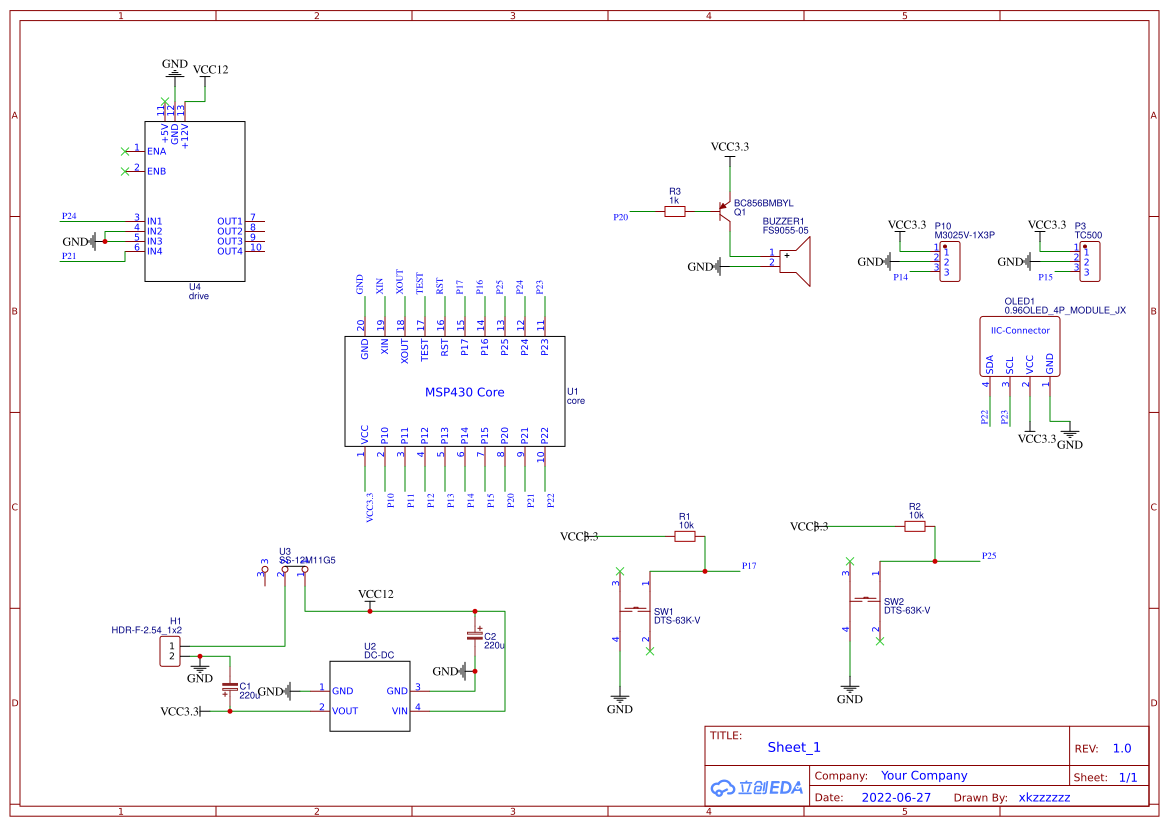
\includegraphics[width=0.5\textwidth]{Schematic.png}
\end{figure}

封装如图~\ref{fig:package},PCB的正反面如图~\ref{fig:pcb}。实物图如图~\ref{fig:real}。

\begin{figure}[htbp]
	\centering
	\caption{封装}
	\label{fig:package}
	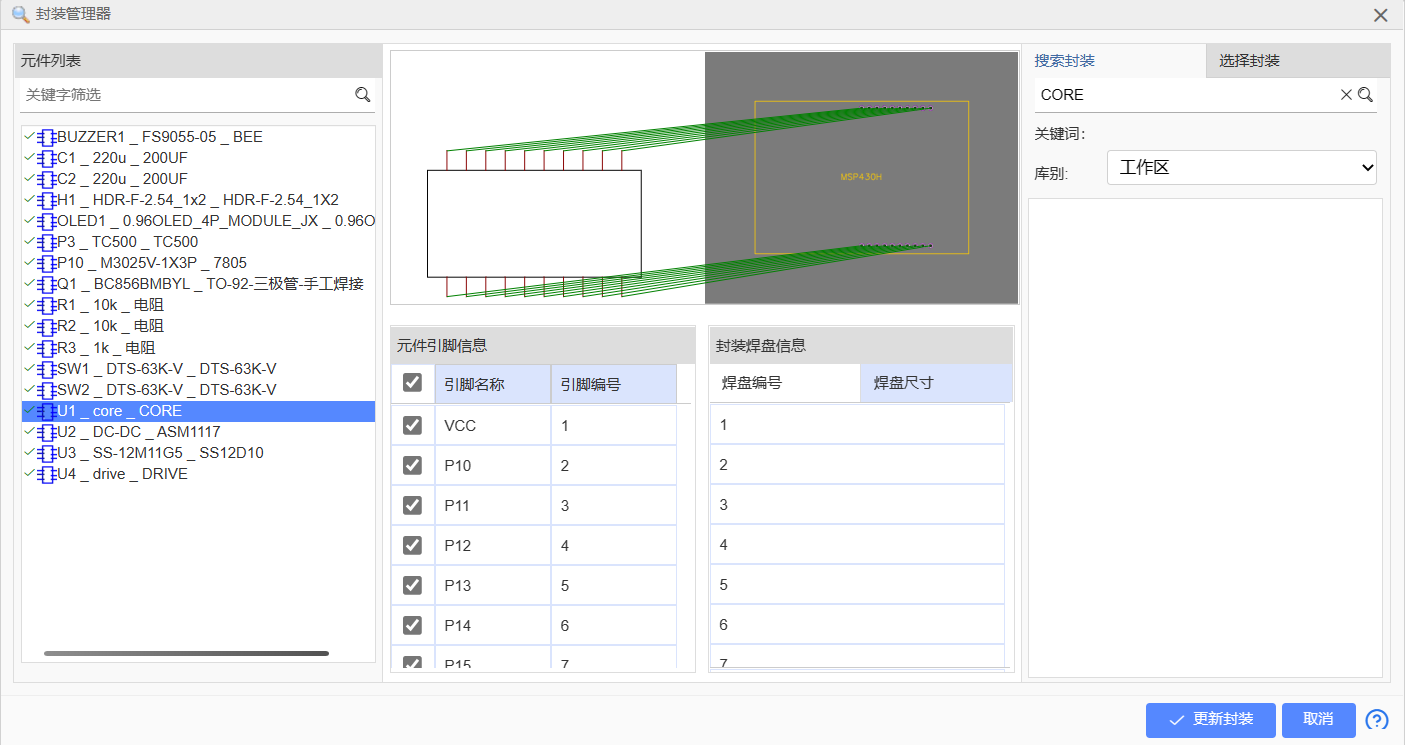
\includegraphics[width=0.6\textwidth]{package.png}
\end{figure}


\begin{figure}[htbp]
    \centering
	\caption{PCB}
	\label{fig:pcb}
	\subfigure[顶部]{
		\begin{minipage}[t]{0.48\linewidth}
			\centering
			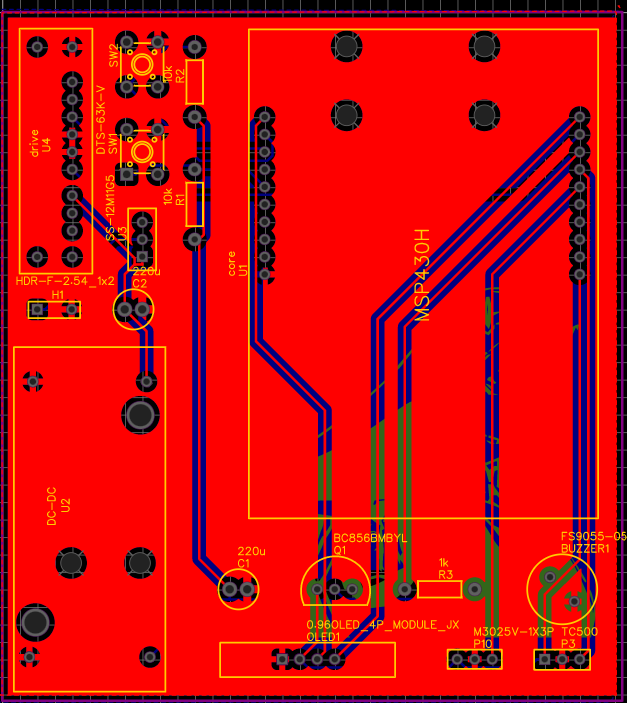
\includegraphics[width=0.8\textwidth]{pcb_top.png}
	\end{minipage}}
	\subfigure[底部]{
		\begin{minipage}[t]{0.48\linewidth}
			\centering
			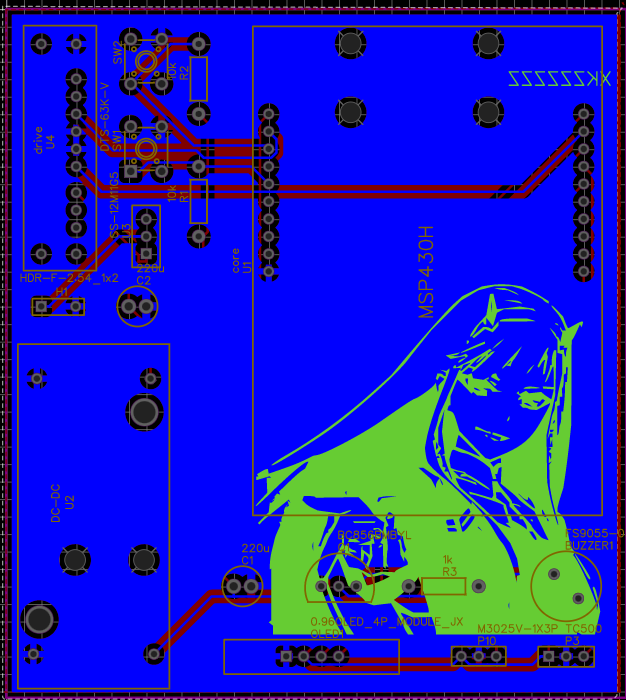
\includegraphics[width=0.8\textwidth]{pcb_bottom.png}
	\end{minipage}}
\end{figure}

\begin{figure}[htbp]
	\centering
	\caption{实物图}
	\label{fig:real}
	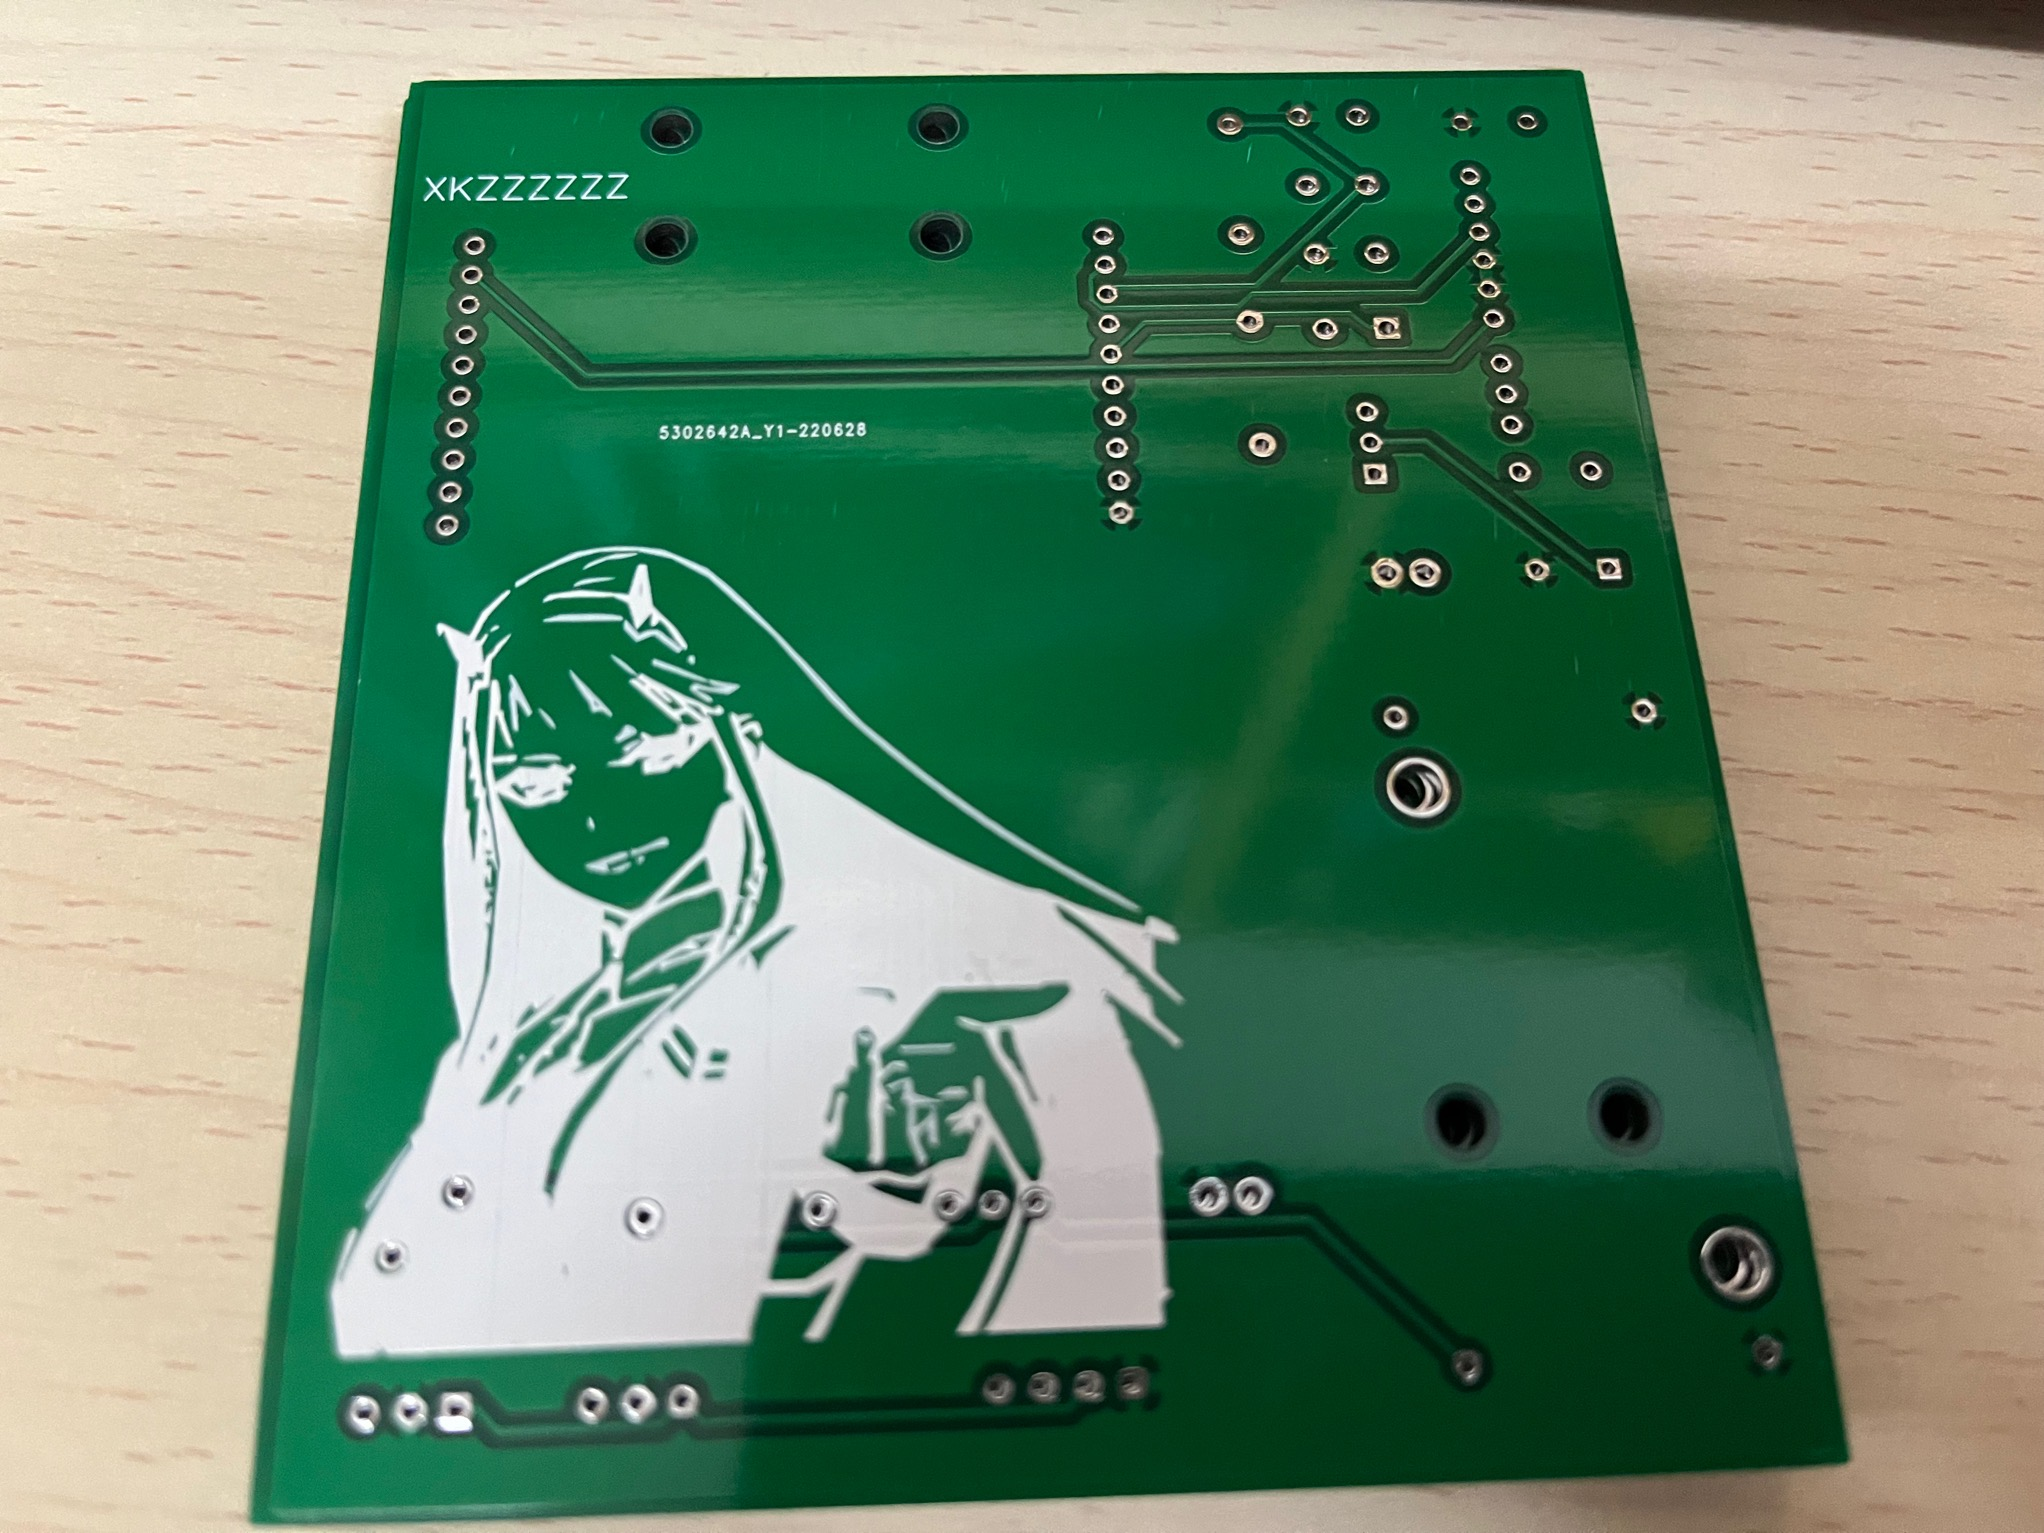
\includegraphics[width=0.6\textwidth]{real.jpg}
\end{figure}


\clearpage
\subsection{注意事项}

\begin{enumerate}
	\item 需要插接导线或者其它线缆的接口元器件一般放到电路板的外侧,
	并且接线的一面要朝外。例如,P1主控板插针一般放到电路板的外侧,
	使单片机接上后多余的部分露在外侧,减少占用PCB板空间。

	\item 元器件就近原则。元器件就近放置,可以缩短PCB导线的距离,
	如果是去耦电容或者滤波电容,越靠近元器件,效果越好。
	例如,H5和SW1就近放置,可以缩短PCB导线距离。

	\item 整齐排列。一个IC芯片的辅助电容电阻电路,围绕此IC把电阻电容整齐的排列,
	可以更美观。例如,R6、R7和C10、C8整齐排列,使整个电路板美观。

	\item 在排列放置元件时,要考虑到实际安装的要求,避免把针脚画反导致需要用线搭接。
\end{enumerate}

\section{MSP430单片机部分}

\subsection{作业1}

\subsection{作业2}

\subsection{作业3}

\subsection{作业4}

\subsection{作业5}

\subsection{作业6}

\section{基于MSP430的智能小车行驶}

\subsection{电路与程序设计}

\subsection{测试方案与测试结果}

\subsection{本人所做的工作}

\subsection{经验总结与个人感受}


\section{人工智能入门}


\section{实验改进建议}


\section{实训总结}


\end{spacing}

\end{document}